\chapter{Experiment and Result}
brief of experiment and result.
\section{Experiment}
Please tell how the experiment conducted from method.

\section{Result}
Please provide the result of experiment

\section{Aip Suprapto Munari/1164063}

\subsection{Teori}
\begin{enumerate}
\item Klasifikasi teks
	\par Klasifikasi teks atau kategorisasi teks merupakan proses yang secara otomatis menempatkan dokumen teks ke dalam suatu kategori berdasarkan isi dari teks tersebut. 
	\begin{figure}[ht]
		\centering
		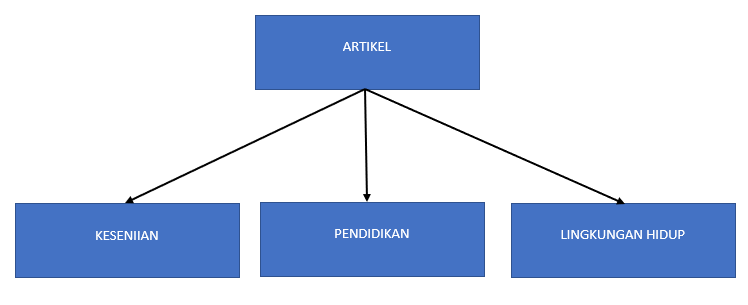
\includegraphics[scale=0.5]{figures/AIP/b1.PNG}
		\caption{Aip-Klasifikasi teks}
		\label{contoh}
	\end{figure}
	
\item Klasifikasi Bunga tidak dapat penggunakan machine learning
	\par Dikarenakan masalah dari input yang serupa namun output yang berbeda ‘noise’, yang dimaksud dengan noise adalah contoh pada output yang direkam bukan seperti perkiraan.
	\begin{figure}[ht]
		\centering
		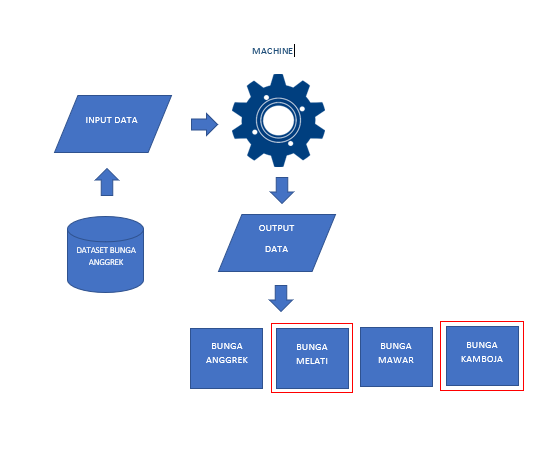
\includegraphics[scale=0.5]{figures/AIP/b2.PNG}
		\caption{Aip-Klasifikasi bunga}
		\label{contoh}
	\end{figure}

\item Teknik pembelajaran mesin pada teks YouTube
	\par Teknik Machine Learning pada YouTube memperhatikan apa saja yang menarik perhatian para penggunanya. Ketika kita sedang menonton di YouTube, pada sebelah kanan terdapat 'Up Next' yang menampilkan beberapa video serupa yang sedang ditonton. Dan ketika mengklik salah satu video dari baris tersebut, maka YouTube akan mengingatnya dan menggunakan kata yang tertera sebagai referensi.
	\begin{figure}[ht]
		\centering
		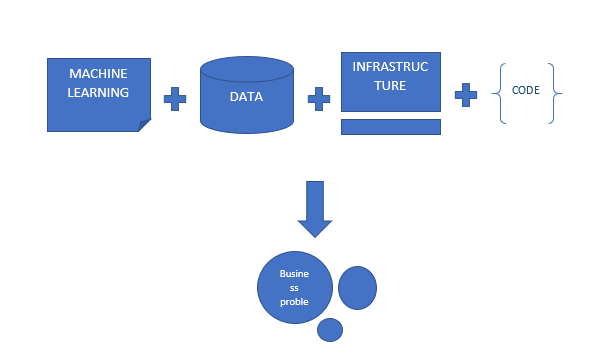
\includegraphics[scale=0.5]{figures/AIP/b3.PNG}
		\caption{Aip-Teknik YouTube}
		\label{contoh}
	\end{figure}

\item Vectorisasi Data
	\begin{itemize}
		\item Vectorisasi Data merupakan pemecahan serta pembagian data kemudian dilakukan perhitungan datanya.
	\end{itemize}
	
\item Bag of word
	\par Bag of Words adalah metode untuk mengekstraksi fitur dari dokumen teks.
	\begin{figure}[ht]
		\centering
		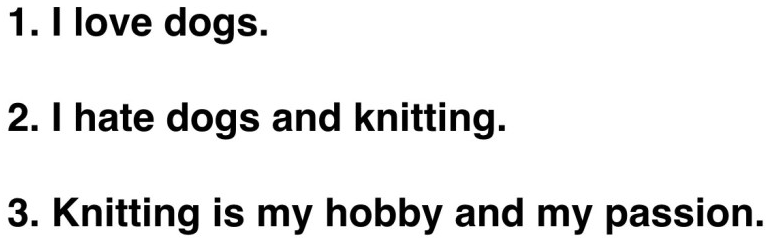
\includegraphics[scale=0.5]{figures/AIP/b4.PNG}
		\caption{Aip-Bag of Word}
		\label{contoh}
	\end{figure}
	
\item TF-IDF
	\par TF-IDF merupakan istilah beberapa frekuensi dokumen terbalik, adalah ukuran penilaian yang banyak digunakan dalam pengambilan informasi (IR) atau peringkasan. 
	\begin{figure}[ht]
		\centering
		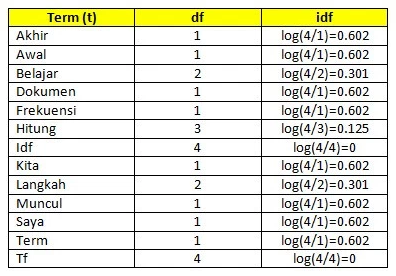
\includegraphics[scale=0.5]{figures/AIP/b5.PNG}
		\caption{Aip-TF IDF}
		\label{contoh}
	\end{figure}
\end{enumerate}